\documentclass{scrartcl}
\usepackage{ucs} 
\usepackage[utf8]{inputenc}  
%\usepackage{ngerman}
\usepackage{cite}
\usepackage{graphicx}

% Do not modify the next 10 lines
% ------------------------------

\usepackage{amssymb,amsmath,url}
\topmargin -0.5in
\footskip 0.7in
\textwidth 6.5in
\textheight 9.0in
\oddsidemargin 0.1in
\evensidemargin 0.1in
\parindent0pt\parskip1ex
% ------------------------------
\usepackage{graphicx}
\graphicspath{ {images/} }
\usepackage{float}
\usepackage{url}

\begin{document}
\title{Master Thesis:\\ Computing Distributed Representations for Polysemous Words}
\author{Haiqing Wang \\Matriculation number: 340863 \\ Advisors:  \\ Dr. Gerhard Paaß \\ Dr. Jörg Kindermann \\ }
\maketitle

\section{Motivation}
\paragraph{}
\hfill \\
Machine learning approaches for natural language processing have to represent the words of a language in a way such that Machine Learning approaches may process them. \\
\\
Recently word representations have been developed which represent each word as a vector of k real numbers (Collobert \& Weston 2008, Mikolov et al. 2013). Generally, we name this process word embedding. By using a large input corpus in an unsupervised algorithm word representations may be derived such that words with similar syntax and semantics have representations with a small Euclidean distance. In subsequent analyses these word representations may be employed for further analyses like opinion mining(Socher et al. 2013, Kim 2014, Tang et al. 2014) or semantic role labeling (Zhou et al. 2015).\\
\\
Note that each word is mapped to a single representation. It is well known, however, that many words may have different meanings, i.e. are polysemous. For example, the word chicken may designate: (1) a domestic fowl, (2) the flesh of a chicken used for food, or (3) a person who lacks confidence. Obviously each of these meanings should be represented by a separate word vector.\\
\\
The main aim of this thesis is to derive expressive word representations for different senses in an efficient way. We will investigate sense assignment models which will extend known word embedding(one sense) approaches, e.g. Senna and Word2Vec (Collobert \& Weston 2008, Mikolov et al. 2013). During learning each word in an sentence is repeatedly assigned to a sense, taking into account the senses of neighboring words. \\

\section{Related works}
\paragraph{Word Embedding}
\hfill \\
There is a very important assumption that if context of words are similar, their representations should be similar as well. So most of methods make use of the context of words to generate vectors.\\
\begin{figure}[H]
\centering
\begin{minipage}{1.0\textwidth}
 
	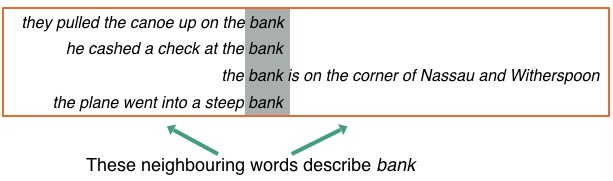
\includegraphics[width=1.0\textwidth]{neighbouring_words} 
	
	\label{fig:neighbouring_words}
\end{minipage}%
\end{figure}	
Traditional approach is word co-occurrence matrix factorization. Each row of the matrix represent the information of one word's context, which is sparse and huge. And then the matrix is decomposed using SVD to generate denser and smaller vectors. The context can be the occurrences in different documents or be the average occurrence's of surrounding words from all documents.  \\
\\         
Recently, artificial neural network is very popular to generate word representations. Prominent algorithms are Senna (Collobert \& Weston 2008) and Word2vec (Mikolov et al. 2013). They both use random initialized vectors to represent words and update the vectors in unsupervised learning: predict a word from the context and update the word vectors according to the score of predicting. The context can be the vector of single surrounding word or the average vector of all surrounding words.\\

\paragraph{Multi-sense Word Embedding}
\hfill \\
One is using clustering of precomputed one-sense word embeddings and their neighborhood embeddings according to (Huang, et al. 2012). The resulting word senses are fixed to the corresponding word neighborhoods and their values are trained until convergence. A similar approach is described in (Chen et al. 2014).\\
\\
Instead of a single embedding each word is represented by a number of different embeddings. During each iteration of the supervised training of Senna or Word2vec for each position of the word the best fitting embedding is selected according the fitness criterion. Subsequently only this embedding is trained using back-propagation. Note that during training a word may be assigned to different senses thus reflecting the training process. A related approach was proposed by (Tian et al. 2014).\\


\section{Approach}
\hfill \\
In this thesis we will investigate sense assignment models which will extend known approaches, e.g. Word2Vec and Senna. During learning each word in an sentence is repeatedly assigned to a sense, taking into account the senses of neighboring words.

\paragraph{Word2Vec}
\hfill \\
Word2Vec is not only a model. Instead, it is a system. There are two different models in Word2Vec: CBOW(continues bag-of-words) model and Skip-gram model. CBOW is to maximize $\prod_{w\in\textit{C}} p(w|context(w))$, and
Skip-gram model is to maximize $\prod_{w\in\textit{C}} \prod_{u\in Context(w)} p(u|w) $ ($\textit{C}$ means Corpus). Input is word vectors initialized randomly, output is probabilities of concern words. Both models use maximum-likelihood estimation with stochastic gradient descent to estimate parameters of models and word vectors.
\begin{figure}[H]
\centering
\begin{minipage}{.5\textwidth}
 
	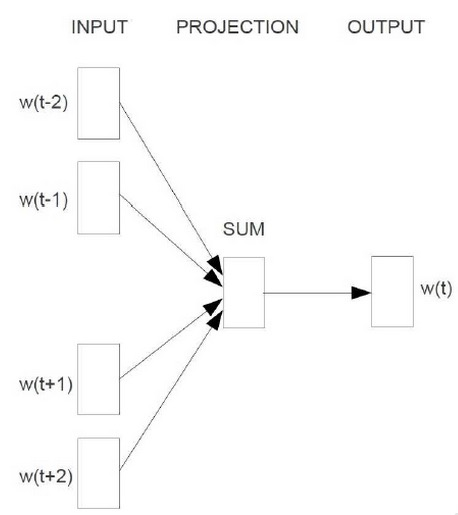
\includegraphics[width=0.9\textwidth]{CBOW} 
	\caption{CBOW model}
	\label{fig:CBOW}
\end{minipage}%
\begin{minipage}{.5\textwidth}
  
	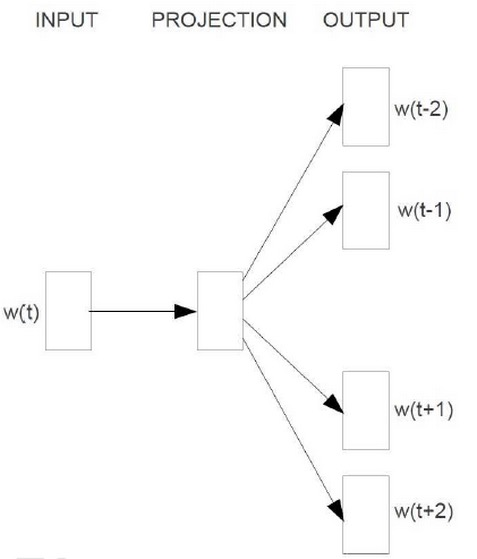
\includegraphics[width=0.85\textwidth]{Skip-Gram}
	\caption{Skip-Gram model}
	\label{fig:Skip-Gram}
\end{minipage}
\end{figure}	

word2vec: 
$$G=\prod_{w_\in C} $$
 
\paragraph{Extend Word2Vec}
\hfill \\
We will use sense vectors instead of word vectors and each word of a sentence will be assigned one sense. Different sense assignment in a sentence can get different score. We will try different score functions for sense assignment and update the assignment in the training. \\
\\
In the process of extending Word2Vec, we will focus on Skip-Gram model. There are some open sources about Word2vec. We can use these codes to extend. In the predicting layer, they uses hierarchical softmax or negative sampling (techniques for accelerating learning) which only support one-sense word. Also original Word2Vec has nothing about sense assignment. So our main tasks are to change the structure of predicting layer and design a structure to support sense assignment. \\

\paragraph{Further Improvement}
\hfill \\
A difficult question is to decide on the number of word senses to use for each word. All approaches derive scores to optimize the representations. We will use the variability of score differences for a word in the corpus to determine the number of word senses.    \\
\\
Further improvement is mainly about dynamic number of word senses. And we will also try some algorithms to decide the number of word senses.\\

\section{Evaluation}
\paragraph{}
\hfill \\
Word representations at the same time capture the syntax and the semantics of a word. For the syntax a representation should reflect the role and position of a word in the sentence. For semantics a representations should be close to words of the same sense which need not necessarily fit into the specific position in a sentence. It is well known that the inclusion of more sequence information during learning yields a more syntax-oriented representation, whereas information about the rest of the document may improve the semantic-oriented representation.\\
\\
We will evaluate the syntactic and the semantic quality of word embeddings on benchmark corpora, e.g. Semeval-2007 (http://nlp.cs.swarthmore.edu/semeval/tasks/task09/data.shtml) coarse-grained all-words dataset. we will also use Semeval-2007 to do word sense disambiguation(WSD). WSD is identifying which sense of a word (i.e. meaning) is used in a sentence, when the word has multiple meanings.\\
\\
Additionally, we will use our embeddings as features in a subsequent supervised task, e.g. Named Entity Recognition. By comparing the results with and without embeddings the additional information in word embeddings may be assessed.\\

\section{Schedule}

\begin{tabular}{|l||c|c|c|c|c|c|}
\hline
\textbf{Month} & \textbf{11} & \textbf{12} & \textbf{1} & \textbf{2} & \textbf{3} & \textbf{4} \\
\hline
\hline
Literature study & X & & & & & \\
Extend word2vec & X & X & & & & \\
Further Improvement & & X & X & & & \\
Evaluation & & & X & X & & \\
Thesis & & & & X & X & X \\
\hline
\end{tabular}

\hfill \\

In the process of extending Word2Vec, we will focus on Skip-Gram model. Extending the structure of predicting layer and designing structure for sense assignment would take some time. Also, we need time to do experiment and adjust parameters. Further improvement is mainly about dynamic number of word senses. For now, the theoretical things are not so clear. So we also need time to complete this part. In the evaluation, evaluating the quality of word embedding and word sense disambiguation testing won't be difficult, while doing other supervised task like named entity recognition would take some time.
\hfill \\
\hfill \\
\hfill \\
\hfill \\
\hfill \\
\hfill \\

\bibliographystyle{abbrv}
\bibliography{literature}

\begin{thebibliography}{99}

\bibitem{1}
R. Collobert and J. Weston. 
{\sl A unified architecture for natural language processing: Deep neural networks with multitask learning}. 
International Conference on Machine Learning (ICML), 2008. 

\bibitem{2}
Huang E H, Socher R, Manning C D, et al. 
{\sl Improving word representations via global context and multiple word prototypes}. 
Association for Computational Linguistics (ACL), 2012.

\bibitem{3}
Mikolov T, Sutskever I, Chen K, et al. 
{\sl Distributed representations of words and phrases and their compositionality}. 
Advances in neural information processing systems, 2013.

\bibitem{4}
Socher R, Perelygin A, Wu J Y, et al. 
{\sl Recursive deep models for semantic compositionality over a sentiment treebank}. 
Empirical Methods on Natural Language Processing (EMNLP), 2013.

\bibitem{5}
Chen X, Liu Z, Sun M. 
{\sl A unified model for word sense representation and disambiguation}. 
Empirical Methods on Natural Language Processing (EMNLP), 2014.

\bibitem{6}
Tian F, Dai H, Bian J, et al. 
{\sl A probabilistic model for learning multi-prototype word embeddings}.
Proceedings of COLING, 2014.

\bibitem{7}
Kim Y. 
{\sl Convolutional neural networks for sentence classification}. 
Empirical Methods on Natural Language Processing (EMNLP). 2014.

\bibitem{8}
Tang D, Wei F, Yang N, et al. 
{\sl Learning sentiment-specific word embedding for twitter sentiment classification}. 
Association for Computational Linguistics (ACL), 2014.

\bibitem{9}
Zhou J, Xu W. 
{\sl End-to-end Learning of Semantic Role Labeling Using Recurrent Neural Networks}. 
Association for Computational Linguistics (ACL), 2015.

\end{thebibliography}

\end{document}
